{\fontsize{12pt}{22pt} \textbf{Mass and density functions}\par}

\vspace{5mm}

Mass function

The probability mass function (p.m.f.) is the histogram of the distribution, that is:

- x-axis: values

- y-axis: frequency

\vspace{5mm}

Density function

The probability density function (p.d.f.) is the "smooth histogram" of the distribution.

\vspace{5mm}

\begin{center}
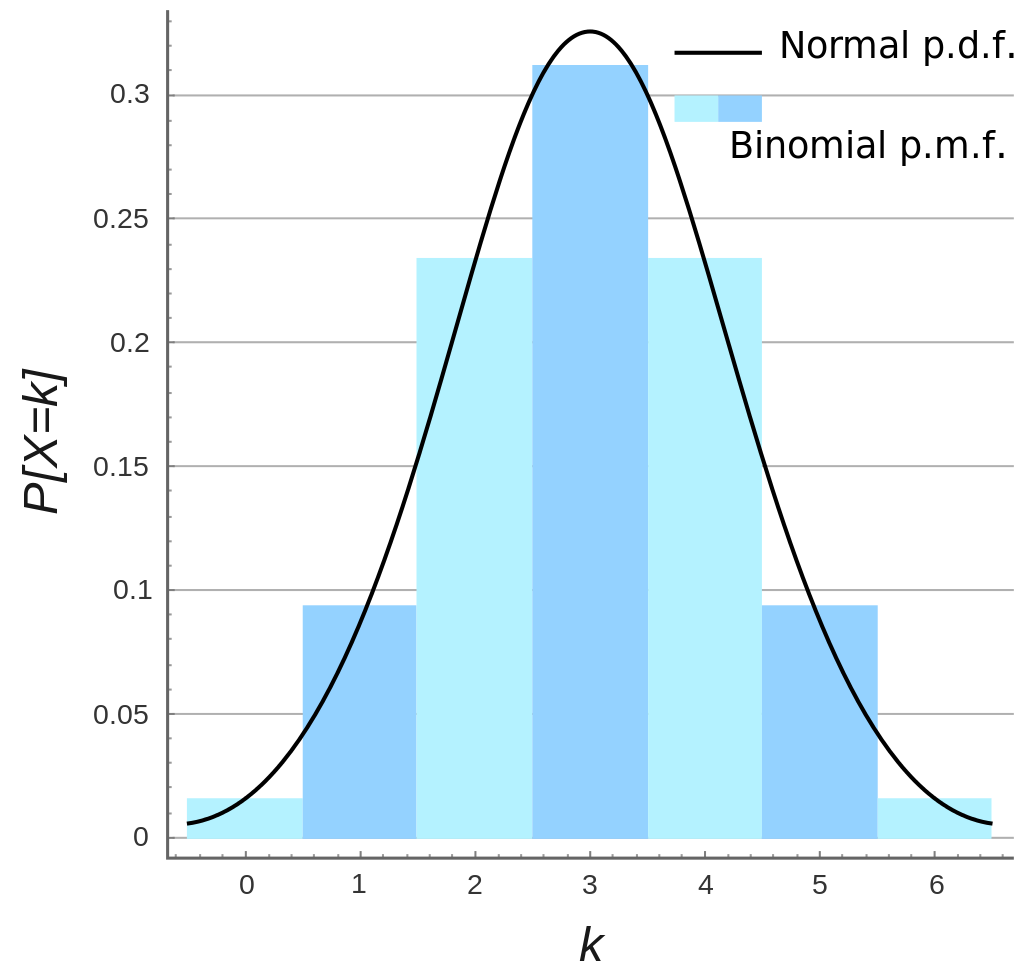
\includegraphics[scale=0.15]{mass_density_functions.png}
\end{center}

\vspace{5mm}